\documentclass[a4paper,11pt]{article}
\usepackage[utf8]{inputenc}
\usepackage[T1]{fontenc}
\usepackage[english,italian]{babel}
\usepackage[pdftex]{graphicx}
\usepackage{tcolorbox}
\usepackage[binary-units]{siunitx}
\usepackage{hyperref}

\usepackage{minted}

\newcommand\source[2]{
	\inputminted[fontsize=\footnotesize,linenos=true,tabsize=4]{#1}{#2}
}

%opening
\title{Interfacciamento di una chitarra e di una pulsantiera ad un PC utilizzando Arduino}
\author{
	Del Duchetto, Francesco\\
	\texttt{francescodelduchetto@gmail.com}
	\and
	Di Luigi, William\\
	\texttt{williamdiluigi@gmail.com}
}

\begin{document}

\maketitle

\begin{abstract}
	La presente relazione descrive i procedimenti che hanno portato gli autori a realizzare un dispositivo elettronico in grado di interfacciare l'uscita analogica di una chitarra elettrica e l'uscita digitale di una pulsantiera con l'ingresso USB di un calcolatore. Il progetto è nato come elaborato nell'ambito del corso di \emph{Programmazione di Sistemi Embedded}.
\end{abstract}

\section{Descrizione sintetica dell'idea del progetto}

Lo scorso anno accademico, Francesco (uno dei due autori) ha sviluppato un software denominato GuitarDSP come elaborato del corso di Programmazione ad oggetti \cite{delduchetto2014}. Questo software permette di applicare, dato un file audio, degli effetti ``in cascata'' dando la possibilità all'utente di scegliere:
\begin{itemize}
\item Quanti effetti applicare: tramite un'apposita interfaccia grafica è possibile aggiungere/eliminare effetti.
\item In che ordine applicare gli effetti: c'è chiaramente una grossa differenza tra applicare un delay dopo una distorsione e applicare invece una distorsione ad un segnale che ha delay.
\item Quali parametri dare a ciascuno degli effetti: ogni effetto espone un'interfaccia che ``istruisce'' la GUI in modo che mostri opportuni slider con i corretti valori minimi e massimi.
\end{itemize}

Il software GuitarDSP è stato concluso e consegnato con successo. Tuttavia, la praticità del suo utilizzo è stata fin da subito gravemente pregiudicata dalla necessità di avere un file audio piuttosto che una connessione diretta tra la chitarra ed il software.

Nella sezione conclusiva della relazione, l'autore di GuitarDSP si proponeva di lavorare ad una ``versione 2.0'' che avrebbe introdotto una modalità di input appositamente studiata per permettere di applicare gli effetti su uno stream ``esterno'' piuttosto che su un file audio. È ora arrivato il momento di implementare questa nuova funzionalità.

\subsection{Aspetti salienti relativamente al corso}

Il software GuitarDSP, essendo sviluppato nell'ambito di un corso di programmazione ad oggetti, implicava la trattazione di aspetti relativi alla buona progettazione del software, al riuso dei componenti, e così via. In questo caso invece, per un elaborato di sistemi embedded, gli aspetti salienti trattati sono:
\begin{itemize}
\item La conversione analogico-digitale: la chitarra produce in uscita un segnale elettrico analogico, che dobbiamo interpretare misurandone la tensione.
\item La comunicazione tra arduino e il PC che elabora gli effetti.
\item La gestione delle problematiche di un sistema \textit{near real time}.
\item La codifica e decodifica di unità di informazione (che contengono il sample audio e il pulsante premuto).
\end{itemize}


\section{Modello semplificato}

Il modello semplificato del progetto realizzato si può descrivere tramite la seguente illustrazione:

\begin{center}
    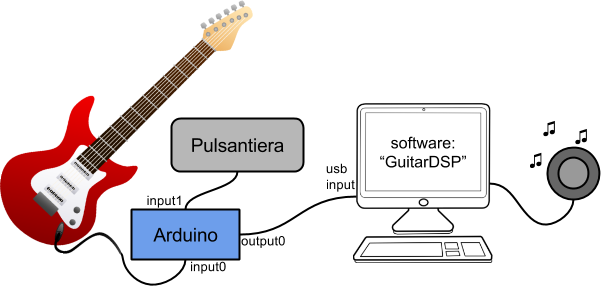
\includegraphics[width=0.9\linewidth]{fig1.png}
\end{center}

Arduino viene usato per interfacciare i dati provenienti dalla chitarra (input0) e dalla pulsantiera (input1) attraverso la porta seriale. L'interfaccia viene poi utilizzata dal software GuitarDSP che elabora l'audio prodotto dalla chitarra applicandogli effetti quali: distortion, reverb, e così via. I dati acquisiti con la pulsantiera vengono utilizzati per decidere quali effetti ``attivare'' o ``disattivare''. Possiamo quindi considerare, nella nostra modellazione, le seguenti entità distinte:\begin{center}
    \begin{minipage}[t]{0.4\textwidth}
        \begin{tcolorbox}
        Un'interfaccia su Arduino che raccoglie i dati dai sensori di input, li elabora e comunica tramite la porta seriale.
        \end{tcolorbox}
    \end{minipage}
    \begin{minipage}[t]{0.5\textwidth}
        \begin{tcolorbox}
        Un'interfaccia sul PC che ascolta le comunicazioni provenienti dalla porta seriale, fa delle elaborazioni e produce un output tramite degli attuatori.
        \end{tcolorbox}
    \end{minipage}
\end{center}

Le due entità agiscono autonomamente, ognuna seguendo i propri obiettivi locali, ma collaborano comunicando tramite il cavo seriale per svolgere un compito globale.

Ciò che stiamo modellando quindi è un sistema multi-agente, composto da due agenti: uno più potente, che si occupa di effettuare i task più dispendiosi a livello di CPU, e l'altro meno potente, che raccoglie i dati dai sensori e li fornisce al primo.

La suddivisione in entità separate rende indipendenti gli agenti coinvolti e permette di estendere il sistema aggiungendone di nuovi senza dover compromettere il funzionamento generale. Ognuno dei due agenti coinvolti non è a conoscenza dei dettagli implementativi e strutturali dell'altro per cui possiamo, ad esempio, sostituire il sottosistema \textsc{Chitarra-Pulsantiera-Arduino} con una tastiera elettronica o un microfono, oppure aggiungere un nuovo algoritmo di elaborazione dell'audio, il tutto senza compromettere la stabilità dell'intero sistema.

L'unica cosa che vincola il comportamento degli agenti è il protocollo utilizzato per lo scambio di informazioni (ovvero il modo in cui i sottosistemi comunicano); fintantoché viene rispettato il protocollo, essi riusciranno con successo a collaborare al funzionamento globale.

\subsection{Requisiti e funzionalità}
I requisiti globali del sistema sono:
\begin{itemize}
    \item ``Ascoltare'' l'audio analogico proveniente dalla chitarra.
    \item Rilevare la pressione dei pulsanti.
    \item Elaborare il suono applicando degli effetti.
    \item ``Suonare'' l'audio risultante con poco ritardo (\textit{near real time}).
    \item Riuscire a gestire una comunicazione efficiente tra le entità.
\end{itemize}

Tutti questi compiti devono essere svolti in modo da rendere usabile il sistema, quindi la latenza tra il suono prodotto dalla chitarra e quello in uscita dal PC non deve essere percettibile e il suono deve essere fedele e coerente con gli effetti selezionati.

\section{Architettura complessiva del sistema}

L'architettura complessiva del sistema creato si può inquadrare nel \textit{Producer-consumer pattern}. Infatti, il sottosistema \textsc{Chitarra-Pulsantiera-Arduino} è un \textit{producer} dal momento che deve creare dei dati, mentre il sottosistema \textsc{Computer} è un \textit{consumer} ed ha il compito di usare i dati che arrivano.

Dopo aver stabilito come il nostro sistema è architettato e i requisiti che deve rispettare, notiamo che per costruirne uno funzionante dobbiamo prima gestire il problema del produttore/consumatore.

\subsection{Problema del produttore/consumatore}
In informatica il problema del produttore/consumatore è un esempio classico di sincronizzazione tra due processi. Il processo \textit{producer} ha il compito di generare continuativamente dei dati, mettendoli di volta in volta in un buffer comune. Il processo \textit{consumer}, dal canto suo, ha il compito di elaborare i dati del buffer estraendoli uno per volta dal buffer.

Nel nostro caso, per garantire un'alta qualità dell'audio, il producer deve generare quanti più dati possibili (magari evitando di eccedere i \num{44100} campioni al secondo, che sono lo standard nelle registrazioni audio). Il consumer, indipendentemente dalla frequenza del producer, consumerà i dati ad una frequenza specifica (decisa in anticipo) che corrisponderà alla frequenza di riproduzione dell'audio.

Come accennato nella sezione precedente, il nostro sistema ha il requisito del near real time. È intuitivo quindi capire che la soluzione al problema del produttore/consumatore è, nel nostro caso specifico, quella di \textit{concordare una frequenza} comune ad entrambi in modo da affaticare il meno possibile il buffer condiviso.

Dal momento che Arduino risulta essere il collo di bottiglia del sistema, a causa del processore a $16$ MHz, è opportuno scegliere la frequenza più alta alla quale il \textit{producer} è in grado di spedire i dati.

\subsection{Campionamento dell'audio}
La lettura dell'audio in input è una funzione cardine del nostro sistema perciò abbiamo speso molto tempo nel cercare il modo migliore per campionare l'audio (per approfondimenti guardare nella sezione \textbf{Test effettuati e discussione}). Visto che la lettura dell'audio è una funzione che deve essere eseguita continuamente, e non ad esempio a fronte di uno specifico evento, ed il più velocemente possibile, abbiamo concluso che la soluzione migliore è quella di usare il convertitore analogico digitale montato sulla scheda. Con l'ADC

\subsection{Applicazione degli effetti e riproduzione dell'audio}

\subsection{Modellazione dei pulsanti}




http://www.arduino.cc/en/Reference/AttachInterrupt

\section{Struttura, comportamento ed interazione delle varie parti}

\begin{itemize}
    \item Sottosistema \textsc{Chitarra-Pulsantiera-Arduino}:
    \begin{enumerate}
        \item Lettura continua dell'audio analogico e campionamento, evitando il più possibile di perdere qualità.
        \item Rilevazione della pressione (asincrona) dei pulsanti.
        \item Spedizione di tutti i dati raccolti tramite l'uscita seriale in modo che arrivino integri al destinatario.
    \end{enumerate}
    \item Sottosistema \textsc{Computer}:
    \begin{enumerate}
        \item Lettura dei dati in arrivo sulla porta USB ``distinguendo'' i dati audio da quelli relativi ai pulsanti.
        \item Elaborazione del suono e applicazione gli effetti.
        \item Modifica della pila di effetti da applicare, in base ai pulsanti premuti.
        \item Invio del suono elaborato sulla linea di output.
    \end{enumerate}
\end{itemize}

\subsection{Circuito elettronico}
Ricordando che i pin analogici di Arduino permettono di leggere valori di tensione compresi tra 0V e 5V, per poter campionare adeguatamente il segnale audio proveniente dalla chitarra abbiamo dovuto gestire due principali problematiche:
\begin{itemize}
    \item Nei segnali audio la tensione assume valori sia positivi che negativi;
    \item il segnale in uscita dalla chitarra non essendo amplificato assume valori di picco dell'ordine dei 200mV, rendendo difficile ricostruire con precisione il segnale.
\end{itemize}

Per questi motivi non possiamo collegare direttamente l'uscita della chitarra ad un pin di Arduino ma dobbiamo progettare e costruire un circuito che trasformi il segnale originario in un segnale adeguato per le esigenze del microcontrollore.
Il circuito deve quindi traslare il segnale nel range 0-5V, centrandolo in 2.5V, e amplificarlo di un fattore circa uguale a 10.

\newpage
Questo è il circuito che abbiamo progettato su Multisim\footnote{\url{http://www.ni.com/multisim/i/}} prima di cablarlo sulla scheda di prototipazione:

\begin{center}
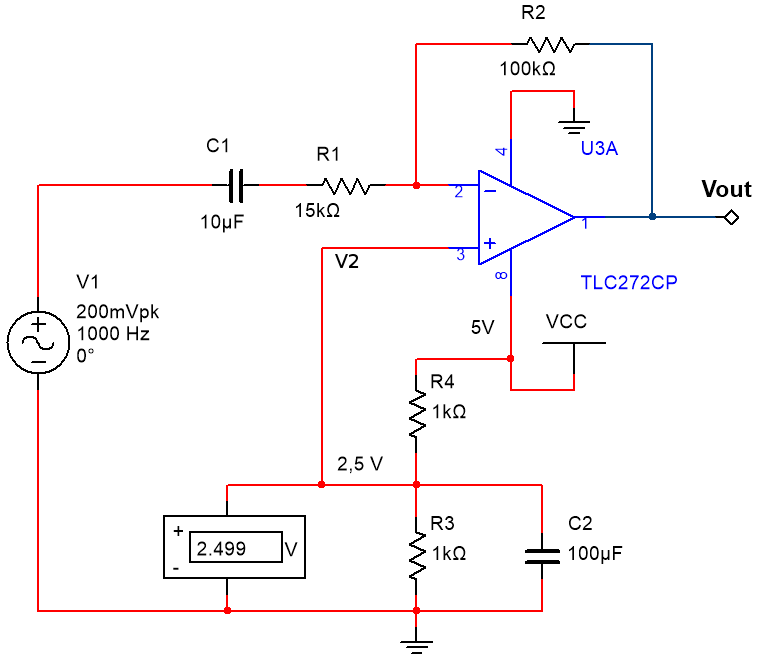
\includegraphics[width=0.9\textwidth]{screen.png}
\end{center}

\texttt{V1} è un oscilloscopio che simula il suono proveniente dalla chitarra.
\texttt{U3A} è un amplificatore operazionale (modello TLC2727CP) collegato in configurazione invertente la cui tensione in uscita sarà: $$Vout = V2 - \frac{R2}{R1} \cdot V1 $$
 
Le resistenze \texttt{R1} e \texttt{R2} quindi servono per regolare il fattore di amplificazione del segnale d'ingresso. Le resistenze \texttt{R3} ed \texttt{R4} sono usate invece per fare un partitore di tensione ed ottenere i 2.5V per spostare il segnale nel range 0-5V.

I condensatori sono stati usati per tagliare via le frequenze di rumore dal segnale di input.

\vspace{0.2in}
\newpage
Nel grafico seguente vediamo in rosso il segnale \texttt{V1} di input e in blu il segnale di output:
\vspace{0.1in}

\begin{center}
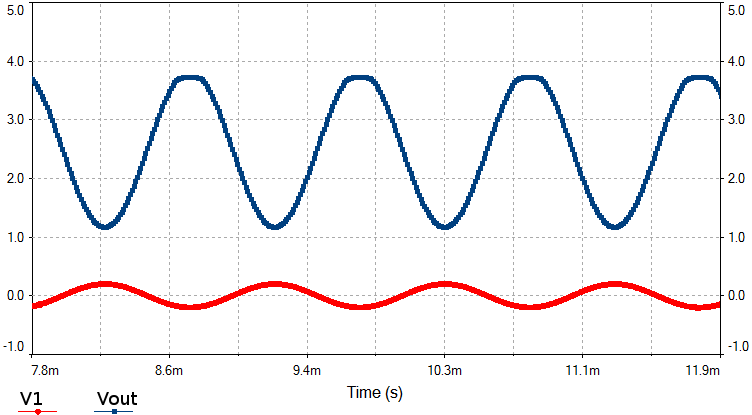
\includegraphics[width=0.9\textwidth]{screen2.png}
\end{center}

Descrizione della struttura/comportamento/interazione delle varie parti.

Utilizzo linguaggi di modellazione appropriati (UML…)

\section{Test effettuati e discussione}

\subsection{Comunicazione Arduino - PC}
La comunicazione tra Arduino e il computer è stato un punto chiave del nostro progetto perchè come vedremo la scelta del protocollo di comunicazione influenza molto le performance del sistema. 

I dati che il microcontrollore deve mandare al computer sono:
\begin{enumerate}
    \item 10 bit dei sample (valori tra 0 e 1024);
    \item notifica della pressione di un pulsante.
\end{enumerate}

\subsubsection{Comunicazione senza overhead}
Il primo testo effettuato e stato quello di non utilizzare nessun protocollo specifico, o meglio mandare i campioni appena raccolti senza aggiungere alcun overhead ai dati. Chiaramente questo approccio è quello che permette la maggior velocità di comunicazione visto che mandiamo solamente i dati utili senza aggiungere nessuna informazione non necessaria.

Naturalmente per scrivere sulla seriale utilizzeremo la funzione \texttt{Serial.write} la quale a differenza di \texttt{Serial.print} non codifica il valore in ASCII, cosa che comporterebbe la spedizione di un pacchetto più grande. La \texttt{Serial.write} può scrivere come minimo valori di byte quindi per scrivere il sample, grande 10 bit, abbiamo bisogno di scrivere due byte. Per i pulsanti invece, che sono 8, ci basta un byte. In totale dobbiamo scirvere 3 byte.

In che ordine scriveremo i nostri byte? E il byte relativo ai pulsanti lo mandiamo sempre o solo quando registriamo una pressione? L'ordine con cui li scriviamo non fa molta differenza, l'importante è che sia ben definito in modo che il computer sappia come interpretare i dati che arrivano. Quindi diciamo che scriviamo prima i due byte del sample (prima il byte più significativo e poi l'altro) ed infine accodiamo il byte dei pulsanti. 
Quest'ultimo byte potremmo decidere di mandarlo solo quando serve, però in che modo il computer riesce a capire quando, dopo i due byte del sample, arriva un byte relativo ai pulsanti e non il primo byte del sample successivo? Senza aggiungere degli ulteriori dati di segnalazione il PC non ha modo di scoprirlo. Allora dobbiamo mandare sempre un pacchetto grande 3 byte, dei quali il terzo conterrà il numero del pulsante premuto se ne è stato premuto uno, o un valore stabilito che indica che non c'è nessuno dato relativo ai pulsanti.
\vspace{0.2in}

Questa soluzione innanzitutto lascia inutilizzato l'ultimo byte per quasi tutta la comunicazione dato che il segnale della pressione si verifica molto di rado rispetto ai sample che vengono mandati di continuo. Ma la vera criticità di questo protocollo è che manca del tutto la sincronizzazione tra mittente e destinatario. Anche assumendo che ogni volta che parte Arduino inizia la comunicazione il computer sia pronto per leggere, e quindi si sincronizza senza errori usando il primo byte arrivato come primo byte di un pacchetto, non è detto che durante la comunicazione questa sincronizzazione non possa essere persa. Se infatti si verificano delle situazioni impreviste (es: Arduino viene riavviato, il cavo si stacca, etc) quando viene ristabilita la comunicazione il primo byte che arriva sulla porta seriale del computer corrisponde al primo byte di un pacchetto? Non è detto. In situazioni del genere il PC continua a leggere e a fare il suo lavoro ignaro del fatto che i dati che sta usando possono non essere quelli corretti.

Per avere un sistema fault-tolerant siamo perciò obbligati ad inserire delle informazioni di sincronizzazione aggiuntive al nostro pacchetto.

\subsubsection{Comunicazione con overhead}
Iniziamo con l'analizzare il contenuto dei byte nel nostro pacchetto:

\begin{table}[h]
\begin{tabular}{ccc}
\textsc{high sample}           & \textsc{low sample}           & \textsc{button}                             \\ \hline
\multicolumn{1}{|c|}{$0\, 0\, 0\, 0\, 0\, 0\, ?\, ? $} & \multicolumn{1}{c|}{$?\,?\,?\,?\,?\,?\,?\,?$} & \multicolumn{1}{c|}{$0\,0\,0\,0\,?\,?\,?\,?$} \\ \hline
\multicolumn{3}{c}{$? \in \{0, 1\}$} 
\end{tabular}
\end{table}

I primi 16 bit del pacchetto (che rappresentano il sample) sono composti sempre da 6 zeri seguiti da 10 cifre qualunque. Il terzo byte è invece formato da 4 zeri seguiti da 4 valori qualunque, perchè i pulsanti sono 8 e 4 bit bastano per scrivere i numeri da 0 a 8.

Osservando come è formato il pacchetto notiamo che possiamo eliminare del tutto il terzo byte, inserendo i 4 bit utili per l'informazione nello spazio libero del primo byte.

\begin{table}[h]
\begin{tabular}{cc}
\textsc{{\color[HTML]{FE0000}button} + high sample}           & \textsc{low sample}       \\ \hline
\multicolumn{1}{|c|}{${\color[HTML]{FE0000}?\,?\,?\,?}\, 0\, 0\, ?\, ? $} & \multicolumn{1}{c|}{$?\,?\,?\,?\,?\,?\,?\,?$} \\ \hline
\multicolumn{2}{c}{$? \in \{0, 1\}$} 
\end{tabular}
\end{table}

Questo ci permette, come vedremo in seguito, di poter campionare ad una frequenza maggiore.
\vspace{0.2in}

Per quanto riguarda la sincronizzazione dobbiamo inserire in testa al nostro pacchetto dei bit aggiuntivi che siano univoci all'interno dello stesso, in modo che il ricevente sappia stabilire con certezza, per ogni pacchetto ricevuto, quale sia il primo byte e quale il secondo. 
Osservando il contenuto del pacchetto possiamo dire che nel primo byte non potremmo mai ottenere il valore 255 (11111111b) dato che ci sono due bit sempre a 0, il secondo byte invece può contenere qualunque valore. A causa del secondo byte dobbiamo inserire due byte di sincronizzazione perchè se ne mettessimo uno potrebbe accadere che il secondo byte (del sample) venga scambiato per esso. 
Quindi inseriamo, in testa al pacchetto originario, due byte di sincronizzazione entrambi con valore 255.

\begin{table}[h]
\begin{tabular}{cccc}
\textsc{\color[HTML]{FE0000}sync} & \textsc{\color[HTML]{FE0000}sync} & \textsc{button + high sample} & \textsc{low sample}       \\ \hline
\multicolumn{1}{|c|}{\color[HTML]{FE0000}$1\,1\,1\,1\, 1\, 1\, 1\, 1 $} &\multicolumn{1}{|c|}{\color[HTML]{FE0000}$1\,1\,1\,1\, 1\, 1\, 1\, 1 $} &\multicolumn{1}{|c|}{${?\,?\,?\,?}\, 0\, 0\, ?\, ? $} & \multicolumn{1}{c|}{$?\,?\,?\,?\,?\,?\,?\,?$} \\ \hline
\multicolumn{2}{c}{} & \multicolumn{2}{c}{$? \in \{0, 1\}$} 
\end{tabular}
\end{table}

Ora da PC siamo sicuri che appena leggiamo due volte 255 seguito da un altro valore, diverso da 255, quest'ultimo è il primo byte del nostro pacchetto originario.

\subsection{Frequenza di campionamento}
La frequenza di campionamento è il numero di campioni prelevati al secondo e si misura in Hertz (\si{\hertz}).
La scelta della frequenza di campionamento del segnale audio è un fattore molto importante nella nostra applicazione per ottenere in uscita una buona qualità audio. Considerando che nei CD audio è uguale a \SI{44.1}{\kilo\hertz} mentre nelle linee telefoniche è \SI{8}{\kilo\hertz}, possiamo dire che per noi una frequenza accettabile si aggira tra questi due, avvicinandosi il più possibile alla prima.

Notare che nel nostro progetto il frame rate che utilizziamo per aprire una linea audio di output è la stessa frequenza di campionamento con cui prendiamo il segnale della chitarra con Arduino, se così non fosse il suono che ne verrebbe fuori, senza applicare nessun effetto, non sarebbe uguale a quello suonato. Per questo motivo è stato importante per noi riuscire a fare una stima abbastanza precisa della frequenza con cui prendiamo l'audio.

Cercheremo ora di stimare che frequenze riusciamo ad ottenere utilizzando Arduino.

\subsubsection{analogRead}
Inizialmente abbiamo provato ad implementare il campionamento audio nel modo più immediato, cioè usando la funzione \texttt{analogRead} fornita dalle librerie di Arduino. 
Abbiamo subito notato che facendo in questo modo dovevamo impostare, quando richiedevamo la linea di output sul PC, un frame rate di circa \SI{5100}{\hertz} per sentire in uscita un suono coerente con quello suonato.

Facendo un po' di prove abbiamo visto che per leggere un campione, utilizzando \texttt{analogRead}, impieghiamo circa \SI{108}{\micro\second} mentre servono \SI{76}{\micro\second} per scrivere sulla linea seriale un pacchetto di \SI{32}{\bit}. 

\source{cpp}{write_speed_rel}

\textit{Con questo sketch abbiamo calcolato il tempo che Arduino impiega per scrivere un pacchetto sulla seriale utilizzando la funzione \texttt{Serial.write}. La funzione \texttt{micros} ritorna il tempo passato dall'avvio di Arduino in microsecondi, con una precisione di 4 microsecondi.}
\vspace{0.2in}

In totale quindi, per leggere dal pin \texttt{A0} e scrivere sulla seriale impieghiamo circa \SI{184}{\micro\second}.
Il processore di Arduino lavora ad una frequenza di \SI{16}{\mega\hertz} (ovvero \num{16e6} cicli al secondo), quindi in \SI{1}{\micro\second} (\SI{e-6}{\second}) esegue \num{16} cicli. Allora il nostro ciclo di campionamento impiega $\num{16 x 184} = \num{2944}$ cicli del processore.

Questo vuol dire che la frequenza massima che possiamo ottenere in questo modo è $\num[quotient-mode = fraction]{16e6 / 2944} = \SI{5434}{\hertz}$, che coincide circa con il valore del frame rate che avevamo trovato empiricamente.
Chiaramente \SI{5}{\kilo\hertz} non sono accettabili per i nostri requisiti, essendo addirittura peggiore della qualità audio telefonica, quindi dobbiamo prendere un'altra strada.

\subsubsection{Analog Digital Converter}
Con Arduino abbiamo la possibilità di sfruttare il convertitore analogico-digitale integrato nella scheda, controllandolo a basso livello.

Il seguente codice attiva l'ADC:
\source{cpp}{adc_setup_rel}

Alla riga \texttt{12} impostiamo il prescaler per la frequenza di campionamento. Il prescaler è un fattore di divisione che va applicato alla frequenza del processore (\SI{16}{\mega\hertz}), e serve per limitare la velocità con cui l'ADC deve lavorare.

La seguente tabella mostra i valori che possiamo scegliere con le relative frequenze e periodi di campionamento:

\begin{table}[h]
\centering
\begin{tabular}{|l|l|l|}
\hline
\textbf{prescaler} & \textbf{frequenza} & \textbf{periodo} \\ \hline \hline
2 & $\SI{8}{\mega\hertz} / 13 \simeq \SI{615.38}{\kilo\hertz}$ & $\SI{1.62}{\micro\second}$\\ \hline
4 & $\SI{4}{\mega\hertz} / 13 \simeq \SI{307.69}{\kilo\hertz}$ & $\SI{3.25}{\micro\second}$\\ \hline
8 & $\SI{2}{\mega\hertz} / 13 \simeq \SI{153.84}{\kilo\hertz}$ & $\SI{6.5}{\micro\second}$\\ \hline
16 & $\SI{1}{\mega\hertz} / 13 \simeq \SI{76.92}{\kilo\hertz}$ & $\SI{13}{\micro\second}$\\ \hline
32 & $\SI{500}{\kilo\hertz} / 13 \simeq \SI{38.46}{\kilo\hertz}$ & $\SI{26}{\micro\second}$\\ \hline
64 & $\SI{250}{\kilo\hertz} / 13 \simeq \SI{19.23}{\kilo\hertz}$ & $\SI{52}{\micro\second}$\\ \hline
128 & $\SI{125}{\kilo\hertz} / 13 \simeq \SI{9.61}{\kilo\hertz}$ & $\SI{104}{\micro\second}$\\  \hline
\end{tabular}
\end{table}

Il valore $13$ che divide ulteriormente la frequenza è il numero di cicli (del clock dell'ADC) che il convertitore impiega per leggere un nuovo valore.

Osserviamo che riusciamo ad ottenere frequenze molto alte, anche molto più di quello di cui abbiamo bisogno. Questo risultato ci potrebbe portare a scegliere il valore minimo per il prescaler al fine di ottenere una qualità altissima dell'audio. Purtroppo non è tutt'oro quel che luccica perchè dobbiamo considerare che aumentando la frequenza cresce il "rumore" nei valori letti sul pin e quindi invece di migliorare la qualità del suono la peggioreremmo. In ogni caso a noi va più che bene un prescaler uguale a 32 che ci da una qualità molto vicina a quella dei CD audio.

Ora dobbiamo però tener conto di un altro fattore che potrebbe limitare la nostra velocità di campionamento: la comunicazione seriale.
Come detto in precedenza i dati raccolti con Arduino devono essere spediti al computer tramite il cavo seriale, quindi se non riusciamo a mandare in tempo tutti i dati che leggiamo siamo comunque costretti ad abbassare la frequenza dell'ADC.

Nelle riga \texttt{14} del codice attiviamo l'interrupt handler del convertitore, questo vuol dire che ogni appena il convertitore avrà finito di leggere un valore chiamerà una funzione che possiamo definire noi. Il codice che inseriremo nella funzione sarà eseguito in sezione critica perciò dobbiamo stare attenti a non inserire cicli molto lunghi e computazioni pesanti in termini di CPU.

La macro \texttt{ISR} marca la funzione come interrupt handler, in questo caso (\texttt{ADC\_vect}) per l'avvenuta lettura del valore da parte dell'ADC.

\source{cpp}{adc_interrupt_rel}

Nella funzione noi leggiamo i valori che sono stati campionati dai registri \texttt{ADCL} e \texttt{ADCH}, li inseriamo nel pacchetto e poi li scriviamo sulla seriale. Assumendo che l'operazione più costosa sia la scrittura sulla porta seriale calcoliamo quanto costa scrivere un pacchetto di 4 byte e consideriamo tale valore come lower bound per il costo del nostro interrupt handler.

Il costo per scrivere un pacchetto di 4 byte, che avevamo trovato nel paragrafo precedente, è in media \SI{76}{\micro\second}. Riguardando la tabella nella pagina precedente leggiamo che campionando a \SI{19.23}{\kilo\hertz} l'ADC legge un nuovo sample ogni \SI{52}{\micro\second}. Impostando perciò un prescaler minore di 128 l'ADC non riuscirà a leggere ogni volta che gli tocca perchè, ricordando che l'interrupt handler esegue in sezione critica, l'handler di gestione dura di più del tempo di attesa tra la lettura di un campione e l'altro ed accadrà che a volte questo metterà in attesa l'ADC che vuole leggere un nuovo sample. 
Questo risultato stronca le nostre speranze sul fatto di ottenere una qualità audio vicina a quella dei CD e ci dice che possiamo ottenere una frequenza che si aggira tra i \SI{19.23}{\kilo\hertz} e i \SI{9.61}{\kilo\hertz}. Empiricamente abbiamo trovato \SI{14.1}{\kilo\hertz} circa.

\vspace{0.2in}
Si potrebbe pensare di lasciare nell'interrupt handler solamente il salvataggio nel pacchetto dei valori letti e scrivere sulla seriale nel loop principale. Questo sicuramente permetterà all'ADC di campionare alla frequenza con cui dovrebbe però noi comunque non riusciremmo a mandare sulla seriale tutti i sample letti, per via del tempo necesario alla scrittura. Anzi peggioreremmo la situazione perchè dato che l'interrupt handler ha priorità maggiore rispetto a quella del loop, prenderà sempre il controllo mentre il loop sta eseguendo facendo satare molti campioni. Facendo una prova abbiamo rilevato una frequenza di campionamento di circa \SI{9}{\kilo\hertz}.

\begin{thebibliography}{9}

\bibitem{delduchetto2014}
  Francesco Del Duchetto,
  \emph{Guitar Effect Processor in Java},
  \url{https://drive.google.com/file/d/0B3icasI9ngtyTko4TDZaYjFDNEE/view},
  2014.

\end{thebibliography}

\end{document}
